\documentclass[10pt,journal,compsoc]{IEEEtran}

\usepackage{amsmath,amssymb,amsfonts}
\usepackage{algorithmic}
\usepackage{graphicx}
\usepackage{textcomp}
\usepackage{xcolor}
\usepackage{booktabs}
\usepackage{multirow}
\usepackage{hyperref}
\usepackage{cite}

\hypersetup{
    colorlinks=true,
    linkcolor=blue,
    citecolor=blue,
    urlcolor=blue
}

\begin{document}

\title{Federated Learning for Resource-Aware Intrusion Detection in IoT Networks: An Empirical Study of IID and Device-Level Non-IID Data}

\author{Moazzam~Azam\\
\IEEEctlauthordNS{Email: moazzamkk13@gmail.com}
}

\markboth{IEEE Transactions on Mobile Computing / IEEE Transactions on Dependable and Secure Computing}%
{Azam: Federated Learning for Resource-Aware Intrusion Detection in IoT Networks}

\maketitle

\begin{abstract}
The proliferation of Internet of Things (IoT) devices has expanded the network attack surface, increasing the risk of botnet-driven intrusions such as Mirai and Gafgyt campaigns. Centralizing raw network traffic from IoT devices for intrusion detection raises data locality concerns and imposes bandwidth costs. Federated learning (FL) offers a decentralized training paradigm in which devices contribute model parameter updates rather than raw data; however, the practical utility of FL for IoT intrusion detection under real-world device-level data heterogeneity has not been empirically characterized with transparent methodology and explicit scope documentation.

This paper presents a controlled empirical study comparing four training conditions on the N-BaIoT dataset: (1) a Centralized baseline, (2) Local-Only isolated training, (3) Federated Averaging (FedAvg) under a natural device-level Non-IID partition, and (4) FedAvg under a controlled class-stratified IID partition. All experiments use a compact feed-forward neural network (\texttt{SmallMLP}, 9,537 parameters) for binary botnet intrusion detection across 9 commercial IoT device types (7,062,606 total observations, 115 features). Experiments were conducted with a single random seed (42) and a 3-round or 3-epoch training horizon.

On the frozen global holdout test set (1,059,388 rows), the Centralized baseline achieved F1=0.9971, Controlled IID FedAvg (Round 3) achieved F1=0.9994, Device-Level Non-IID FedAvg (Round 3) achieved F1=0.9757, and Local-Only models yielded a macro-average F1=0.9714 on local same-device test subsets. Communication payload accounting records a cumulative model parameter exchange of ~1.96 MiB (2,059,992 bytes) across 9 clients over 3 rounds.

The study documents explicit scope boundaries: a single random seed, 3 communication rounds, simulated rather than physical clients, a centrally pre-fitted feature scaler, host CPU resource measurements, and the absence of formal privacy guarantees. The primary contribution is a reproducible empirical comparison of performance, communication payload, and host-side resource characteristics across centralized, federated, and local-only training topologies for IoT intrusion detection.
\end{abstract}

\begin{IEEEkeywords}
Federated learning, IoT intrusion detection, N-BaIoT, FedAvg, non-IID data, device heterogeneity, empirical evaluation, botnet detection.
\end{IEEEkeywords}

\section{Introduction}

\subsection{IoT Security Context}
The adoption of Internet of Things devices—spanning smart home sensors, IP cameras, doorbells, thermostats, baby monitors, and industrial monitoring nodes—has grown substantially over the past decade. These devices maintain persistent network connectivity and often run lightweight embedded operating systems with limited security hardening. As a result, they have become attractive targets for large-scale botnet campaigns. The Mirai botnet, which infected hundreds of thousands of IoT devices and launched distributed denial-of-service attacks exceeding 1 Tbps, demonstrated the severity of the threat; subsequent Gafgyt variants extended infection methodologies and target profiles \cite{meidan2018nbaiot}.

Detecting these intrusions requires monitoring network traffic generated by IoT endpoints. Network-based intrusion detection systems (NIDS) analyze packet header statistics, flow-level features, and temporal traffic patterns to distinguish benign device behavior from malicious activity. Machine learning models trained on labeled traffic samples have demonstrated effectiveness for IoT botnet detection in controlled benchmarks \cite{zarpelao2017survey}, \cite{chaabouni2019network}. However, applying these techniques in practice introduces methodological and deployment challenges that motivate the present study.

\subsection{The Data Centralization Challenge}
Standard supervised machine learning assumes that labeled training data can be pooled at a central location. For IoT network traffic, this assumption is problematic. Network traffic logs may contain sensitive behavioral signals about devices and their users, creating data locality concerns. Transmitting raw traffic data from many distributed IoT endpoints to a central training server consumes network bandwidth, which can be prohibitive for low-bandwidth edge deployments. In multi-organization or multi-tenant environments, separate administrative domains may be unwilling to share raw traffic observations with a central aggregator.

These factors create pressure to develop training approaches that do not require centralizing raw device traffic data for model training.

\subsection{Federated Learning as a Decentralized Alternative}
Federated learning, introduced by McMahan et al. \cite{mcmahan2017communication} as the Federated Averaging (FedAvg) algorithm, offers a decentralized training paradigm: instead of transmitting raw data, each participating client trains a local model copy on its local data partition and transmits only model parameter updates to a central coordinator. The coordinator aggregates these updates into a global model, which is then redistributed to clients for the next training round. This process repeats over successive communication rounds.

By exchanging model parameters rather than raw observations, FL avoids direct data centralization. The FedAvg protocol defines a communication-computation trade-off: reducing communication rounds or decreasing local training epochs reduces parameter exchange frequency but may slow convergence. The compact representation of model parameters—relative to raw training datasets—makes parameter exchange feasible even over constrained network links.

\subsection{The Non-IID Data Heterogeneity Problem}
A critical practical challenge in federated IoT deployments is that client data are not independently and identically distributed (non-IID) across devices. Different IoT device types—cameras, thermostats, doorbells, baby monitors—generate traffic with distinct temporal patterns, packet size distributions, and protocol usage profiles. When each device type constitutes a separate federated client, the local data distributions differ substantially across participants.

Prior theoretical and empirical analyses have demonstrated that non-IID client data can impair FedAvg convergence, increase gradient divergence across clients, and widen the performance gap relative to centralized training \cite{zhao2018federated}, \cite{li2020federated}. Large-scale open problem surveys identify client data heterogeneity as one of the primary challenges for practical FL deployment \cite{kairouz2021advances}. However, the magnitude of the non-IID effect is problem-specific, and empirical studies with transparent methodology and explicit scope documentation are needed to characterize the effect on IoT botnet detection tasks.

\subsection{Research Gap}
Despite the growing body of work on FL and on machine-learning-based IoT intrusion detection, controlled empirical comparisons that systematically isolate the effect of client data distribution—holding model architecture, training configuration, and dataset constant—remain limited. Furthermore, many published studies do not document explicit methodological boundaries (e.g., single-seed variance, simulated vs. physical clients, scaler centralization, communication accounting scope) that are necessary for correct scientific interpretation. This limits reproducibility and creates barriers to fair cross-study comparison.

\subsection{Study Design and Contributions}
This paper addresses the research gap through a controlled empirical study with the following characteristics:
\begin{itemize}
    \item \textbf{Dataset:} The N-BaIoT dataset \cite{meidan2018nbaiot}, comprising 7,062,606 labeled network traffic observations from 9 commercial IoT device types, with 115 continuous features capturing multi-scale temporal traffic statistics.
    \item \textbf{Model:} A compact feed-forward neural network (\texttt{SmallMLP}, $115 \rightarrow 64 \rightarrow 32 \rightarrow 1$, 9,537 trainable parameters), selected to represent a parameter-efficient architecture appropriate for IoT resource profiles.
    \item \textbf{Experimental Conditions:} Four conditions evaluated under a frozen dataset split (seed 42): Centralized baseline, Local-Only isolation, Device-Level Non-IID FedAvg (natural device partitions), and Controlled IID FedAvg (class-stratified redistribution).
    \item \textbf{Explicit Scope:} A single random seed, 3-round/3-epoch training horizon, single-host CPU simulation, centrally pre-fitted feature scaler, theoretical communication payload accounting, and absence of formal privacy guarantees are all documented as scope boundaries rather than omitted.
\end{itemize}

The primary contributions of this study are:
\begin{enumerate}
    \item A reproducible empirical comparison of performance trade-offs across centralized, federated (IID and device-level Non-IID), and local-only training topologies on the N-BaIoT intrusion detection benchmark.
    \item A duplicate-aware frozen dataset split strategy that enforces \texttt{(device, feature\_hash)} grouping within each device partition to prevent intra-device feature-vector data leakage across train/validation/test boundaries.
    \item Transparent communication payload accounting and host-side computational resource characterization, with explicit documentation of accounting scope boundaries.
    \item Explicit documentation of 18 methodological limitations and threats to validity, enabling correct scientific interpretation and supporting reliable replication.
\end{enumerate}

\subsection{Research Questions}
This study is organized around three primary research questions:
\begin{itemize}
    \item \textbf{RQ1 — Performance Under Different Training Topologies:} How does standard Federated Averaging (FedAvg) compare with a centralized training baseline and local-only isolated training in terms of binary intrusion detection performance (F1-Score, ROC-AUC, Accuracy, Precision, Recall, Loss) on the N-BaIoT dataset, under a fixed model architecture, optimizer, and 3-round/3-epoch training horizon?
    \item \textbf{RQ2 — Effect of Client Data Distribution:} How does the choice of client data partition—natural device-level Non-IID assignment versus a controlled class-stratified IID redistribution—affect FedAvg global model performance and early-stage convergence trajectories across communication rounds, when all other experimental parameters are held constant?
    \item \textbf{RQ3 — Communication and Host-Side Resource Characteristics:} What are the model parameter payload communication volumes and host-side computational resource characteristics (peak process-tree RAM, execution wall time) associated with centralized, federated, and local-only training under this experimental configuration?
\end{itemize}

The remainder of this paper is organized as follows. Section~\ref{sec:related} reviews related work. Section~\ref{sec:methodology} details the methodology. Section~\ref{sec:setup} describes the experimental setup. Section~\ref{sec:results} presents empirical results. Section~\ref{sec:discussion} discusses the findings. Section~\ref{sec:limitations} documents limitations and threats to validity. Section~\ref{sec:conclusion} presents conclusions and future work directions.

\section{Related Work and Background}
\label{sec:related}

\subsection{IoT Botnet Intrusion Detection}
The N-BaIoT dataset \cite{meidan2018nbaiot} was constructed by Meidan et al. to enable machine-learning-based detection of Mirai and Gafgyt botnet infections on commercial IoT devices. The dataset captures network traffic statistics across multiple temporal decay windows and aggregation streams, yielding 115 continuous features per observation. Published evaluations using deep autoencoders on N-BaIoT demonstrated high per-device detection accuracy, establishing it as a widely used benchmark for IoT NIDS research.

Zarpelão et al. \cite{zarpelao2017survey} surveyed IDS architectures for IoT environments and identified the challenge of heterogeneous device behavior and constrained hardware as key barriers to effective IDS deployment. Chaabouni et al. \cite{chaabouni2019network} reviewed network-based IDS approaches for IoT, noting that machine learning methods offer strong detection capability but are sensitive to training data quality, feature selection, and dataset representativeness. Both surveys identify centralized data collection for model training as an implicit assumption that may not hold in real-world IoT deployments.

\subsection{Federated Learning Foundations}
McMahan et al. \cite{mcmahan2017communication} introduced Federated Averaging (FedAvg) as a communication-efficient alternative to centralized SGD for training neural networks from decentralized data. FedAvg reduces communication rounds by allowing clients to perform multiple local SGD steps before transmitting updated parameters to the coordinator. The central coordinator aggregates local parameter updates using sample-weighted averaging to produce the next global model. McMahan et al. demonstrated that FedAvg can match centralized training accuracy on several benchmarks while substantially reducing communication iterations.

Li et al. \cite{li2020federated} provided a comprehensive survey of federated learning challenges, methods, and future research directions, identifying communication efficiency, systems heterogeneity, statistical heterogeneity (non-IID data), and privacy as the four primary challenge axes. Kairouz et al. \cite{kairouz2021advances} compiled an extensive open-problems survey covering non-IID partition benchmarks, client selection, privacy-utility trade-offs, and robustness, establishing a reference framework for evaluating FL systems.

\subsection{Non-IID Data Heterogeneity}
Zhao et al. \cite{zhao2018federated} empirically demonstrated that non-IID client data degrades FedAvg convergence relative to IID conditions across convolutional networks on vision benchmarks. The study attributed the performance gap to divergence between client-local gradient directions when local data distributions differ substantially. Li et al. \cite{li2020federated} and Kairouz et al. \cite{kairouz2021advances} corroborated that client statistical heterogeneity is one of the most practically significant challenges for FL deployment.

To address non-IID degradation, several algorithmic alternatives to standard FedAvg have been proposed. Li et al. \cite{li2020federated_prox} introduced FedProx, which adds a proximal term to client local objectives to limit parameter drift from the global model. Karimireddy et al. \cite{karimireddy2020scaffold} proposed SCAFFOLD, which uses control variates to correct for gradient drift across heterogeneous clients. While these methods represent promising future extensions, the present study evaluates standard FedAvg as the baseline federated protocol, with FedProx and SCAFFOLD noted as future comparison directions.

\subsection{Data Leakage in Security Machine Learning}
Arp et al. \cite{arp2022dos} conducted a systematic analysis of methodological pitfalls in security machine learning research, identifying data leakage as a pervasive problem. Leakage arises when test observations are statistically dependent on training observations—for example, when duplicate feature vectors appear across train/test splits, or when preprocessing transformations are fitted on pooled data that includes test observations. The present study implements a \texttt{(device, feature\_hash)} group-level frozen split to prevent duplicate feature vectors from spanning split boundaries, directly addressing the leakage concern identified by Arp et al. \cite{arp2022dos}.

\subsection{Privacy and Security in Federated Learning}
While FedAvg reduces raw data centralization, it does not provide formal privacy guarantees. Dwork \cite{dwork2006differential} established the mathematical foundations of Differential Privacy ($\epsilon, \delta$), providing a framework for quantifying the privacy cost of releasing computed statistics. Abadi et al. \cite{abadi2016deep} demonstrated how Differential Privacy can be incorporated into deep neural network training via DP-SGD, enabling gradient-level privacy accounting. Bonawitz et al. \cite{bonawitz2017practical} introduced practical Secure Aggregation, allowing a central coordinator to compute the sum of client model updates without seeing individual client parameters.

On the adversarial side, Blanchard et al. \cite{blanchard2017machine} analyzed Byzantine-tolerant gradient aggregation, demonstrating that even a small number of malicious clients can corrupt standard gradient averaging. Bhagoji et al. \cite{bhagoji2019analyzing} examined model poisoning attacks against federated learning, showing that adversarial clients can introduce backdoors into the global model through carefully crafted local updates. The present study does not incorporate DP, Secure Aggregation, or defenses against Byzantine or poisoning attacks; these are explicitly documented as scope boundaries (Section~\ref{sec:privacy_scope}) and identified as future research directions (Section~\ref{sec:future_work}).

\section{Methodology}
\label{sec:methodology}

\subsection{Federated Learning Framework and FedAvg Protocol}
The study models federated learning across a set of $K = 9$ logical IoT client participants managed by a central aggregation coordinator. The learning objective is to optimize a global parameter vector $W \in \mathbb{R}^d$ for binary traffic classification without centralizing raw observations.

Federated experiments execute the standard Federated Averaging (FedAvg) algorithm \cite{mcmahan2017communication}. For each communication round $r \in \{1, 2, 3\}$:
\begin{enumerate}
    \item \textbf{Global Model Broadcast:} The central coordinator serializes the global model parameter state dictionary $W^{r-1}$ and distributes a copy to all 9 participating clients.
    \item \textbf{Local Training:} Each client $k \in \{1, \dots, 9\}$ instantiates a local model initialized with $W^{r-1}$ and trains locally for $E = 1$ epoch over its assigned training subset $D_k$ ($n_k = |D_k|$) using the Adam optimizer ($\alpha = 0.001$, batch size 256).
    \item \textbf{State Upload:} Upon local training completion, each client returns its updated parameter state dictionary $W_k^r$ and sample count $n_k$ to the coordinator.
    \item \textbf{Weighted Parameter Aggregation:} The coordinator computes the updated global parameter state dictionary $W^r$ via sample-weighted parameter averaging:
    \begin{equation}
        W^r = \sum_{k=1}^{K} \frac{n_k}{N} W_k^r \quad \text{where } N = \sum_{k=1}^K n_k = 4,943,824, \; K = 9
    \end{equation}
    \item \textbf{Global Model Update:} The global model parameters are updated with $W^r$ to complete the round.
\end{enumerate}

Transmission involves full model parameter state dictionaries (\texttt{state\_dict}), not loss gradients.

\subsection{Duplicate-Aware Dataset Partitioning Strategies}
To systematically analyze client data distribution effects while strictly preventing data leakage \cite{arp2022dos}, two primary client partitioning strategies were established:
\begin{enumerate}
    \item \textbf{Device-Level Non-IID Partition:} The 9 physical IoT device sources are mapped directly to 9 simulated logical federated learning clients. Client dataset sizes reflect natural device traffic proportions, ranging from 248,850 training rows (Ennio Doorbell) to 769,074 training rows (Philips Baby Monitor). This setup models non-identically distributed (Non-IID) data skewed by device functionality and usage patterns.
    \item \textbf{Controlled IID Partition:} The 4,943,824 training observations were redistributed deterministically across 9 simulated logical clients using class-stratified random assignment (seed 42). Each client receives approximately 549,313 to 549,315 training rows with matching benign and attack class proportions. This partition serves as an experimental control to isolate non-IID distribution effects from algorithm behavior.
\end{enumerate}

To prevent intra-device data leakage across split boundaries, partitioning was performed at the \texttt{(device, feature\_hash)} group level within each device partition, ensuring that duplicate feature-vector groups within a device were kept indivisible and assigned exclusively to one split boundary (train, val, or test).

\subsection{Model Architecture (\texttt{SmallMLP})}
All experiments evaluate a lightweight feed-forward Multi-Layer Perceptron (\texttt{SmallMLP}). The architecture consists of:
\begin{itemize}
    \item \textbf{Input Layer:} 115 continuous network traffic features.
    \item \textbf{Hidden Layer 1:} 64 linear units followed by Rectified Linear Unit (ReLU) activation.
    \item \textbf{Hidden Layer 2:} 32 linear units followed by Rectified Linear Unit (ReLU) activation.
    \item \textbf{Output Layer:} 1 linear unit followed by Sigmoid activation, producing an estimated probability $p \in [0, 1]$ of attack traffic.
\end{itemize}

The network contains exactly \textbf{9,537 trainable parameters}, calculated as:
\begin{equation}
\begin{aligned}
\text{Layer 1 Weights and Biases: } (115 \times 64) + 64 &= 7,424 \\
\text{Layer 2 Weights and Biases: } (64 \times 32) + 32 &= 2,080 \\
\text{Output Layer Weights and Biases: } (32 \times 1) + 1 &= 33 \\
\text{Total Parameters: } 7,424 + 2,080 + 33 &= 9,537
\end{aligned}
\end{equation}

Training minimizes Binary Cross-Entropy loss over batch predictions:
\begin{equation}
\mathcal{L}_{BCE} = -\frac{1}{N} \sum_{i=1}^N \left[ y_i \log(\hat{y}_i) + (1 - y_i) \log(1 - \hat{y}_i) \right]
\end{equation}

\subsection{Preprocessing and Standardization Pipeline}
Feature standardization is performed using Scikit-Learn's \texttt{StandardScaler}. Features are transformed to zero mean and unit variance according to:
\begin{equation}
z = \frac{x - \mu}{\sigma}
\end{equation}

In the experimental implementation, \texttt{StandardScaler} was fitted incrementally strictly over the combined 4,943,824 training rows prior to federated partitioning. All validation and test partitions were transformed using these fixed training mean ($\mu$) and standard deviation ($\sigma$) vectors without refitting.

\section{Experimental Setup}
\label{sec:setup}

\subsection{Benchmark Dataset (N-BaIoT)}
This study evaluates intrusion detection models using the N-BaIoT dataset \cite{meidan2018nbaiot}, comprising 7,062,606 network traffic observations collected from 9 distinct commercial IoT device types. The primary task is binary intrusion detection (Class 0: Benign, Class 1: Mirai/Gafgyt attack). The frozen split allocation generated with seed 42 comprises: Training Set: 4,943,824 rows (70.00\%), Validation Set: 1,059,394 rows (15.00\%), and Test Set: 1,059,388 rows (15.00\%).

\subsection{Experimental Topologies and Baselines}
Four experimental conditions were evaluated: (1) Centralized Baseline, (2) Local-Only Baseline (9 isolated per-device models), (3) Device-Level Non-IID FedAvg, and (4) Controlled IID FedAvg.

\subsection{Training and Hyperparameter Configuration}
Models were trained using the Adam optimizer ($\alpha = 0.001$, batch size 256, seed 42) on CPU. Centralized and Local-Only baselines ran for 3 epochs; FedAvg ran for 3 communication rounds with $E = 1$ local epoch per round and full client participation ($C = 1.0$).

\subsection{Evaluation Protocol and Metrics}
Model performance is evaluated across six metrics: Loss, Accuracy, Precision, Recall, F1-Score, and ROC-AUC at a probability threshold of 0.5.

\subsection{Communication Payload Accounting Model}
The \texttt{SmallMLP} state dictionary contains 9,537 float32 parameters, yielding a weight payload of \textbf{38,148 bytes} (~37.25 KiB). Per-client per-round transfer (1 download + 1 upload) is 76,296 bytes. Per-round total across 9 clients is 686,664 bytes (~0.655 MiB). The 3-round cumulative total parameter exchange is \textbf{2,059,992 bytes} (~1.96 MiB).

\subsection{Computational Resource Measurement Protocol}
Resource overhead was measured during process execution via process-tree Resident Set Size (RSS) monitoring using Python \texttt{psutil} sampled at 0.1-second intervals.

\section{Results}
\label{sec:results}

\subsection{Overall Final-Test Performance}
Table~\ref{tab:final_test} summarizes the final holdout test set evaluation across all conditions.

\begin{table*}[t]
\caption{Final holdout test set evaluation results across experimental conditions.}
\label{tab:final_test}
\centering
\begin{tabular}{l c c c c c c c c}
\toprule
\textbf{Experiment} & \textbf{Evaluation Scope} & \textbf{Test Rows} & \textbf{Loss} & \textbf{Accuracy} & \textbf{Precision} & \textbf{Recall} & \textbf{F1-Score} & \textbf{ROC-AUC} \\
\midrule
\textbf{Centralized Baseline} & Global Test Set & 1,059,388 & 0.051443 & 0.994635 & 0.994216 & 0.999994 & \textbf{0.997097} & 0.996899 \\
\textbf{Controlled IID FedAvg (Rd 3)} & Global Test Set & 1,059,388 & 0.005075 & 0.998949 & 0.999193 & 0.999667 & \textbf{0.999430} & 0.999859 \\
\textbf{Device Non-IID FedAvg (Rd 3)} & Global Test Set & 1,059,388 & 0.129260 & 0.954104 & 0.952555 & 0.999990 & \textbf{0.975696} & 0.992387 \\
\textbf{Local-Only (Macro Average)} & Same-Device Subsets & 1,059,388 & 0.313455 & 0.946415 & 0.945825 & 0.999971 & \textbf{0.971422} & 0.994417 \\
\textbf{Local-Only (Weighted Average)} & Same-Device Subsets & 1,059,388 & 0.315096 & 0.943251 & 0.942662 & 0.999976 & \textbf{0.969684} & 0.994566 \\
\bottomrule
\end{tabular}
\end{table*}

On the global test set, Centralized baseline achieved F1 = \textbf{0.997097}, Controlled IID FedAvg reached F1 = \textbf{0.999430}, and Device Non-IID FedAvg reached F1 = \textbf{0.975696}. Local-Only models achieved a macro-average F1 of \textbf{0.971422}.

\subsection{FedAvg Convergence Across Rounds}
Table~\ref{tab:fedavg_convergence} details round-by-round validation metrics.

\begin{table*}[t]
\caption{Global validation performance across communication rounds for FedAvg partitions.}
\label{tab:fedavg_convergence}
\centering
\begin{tabular}{l c c c c c c c c c}
\toprule
\textbf{Partition} & \textbf{Round} & \textbf{Training Samples} & \textbf{Agg. Time (s)} & \textbf{Wall Time (s)} & \textbf{Loss} & \textbf{Accuracy} & \textbf{Precision} & \textbf{Recall} & \textbf{F1-Score} \\
\midrule
\textbf{Device Non-IID} & 1 & 4,943,824 & 0.006371 & 828.88 & 0.828505 & 0.921285 & 0.921285 & 1.000000 & 0.959030 \\
\textbf{Device Non-IID} & 2 & 4,943,824 & 0.004894 & 805.37 & 0.283213 & 0.928603 & 0.928078 & 0.999998 & 0.962697 \\
\textbf{Device Non-IID} & 3 & 4,943,824 & 0.005069 & 778.94 & 0.133517 & 0.954014 & 0.952468 & 0.999989 & 0.975650 \\
\midrule
\textbf{Controlled IID} & 1 & 4,943,824 & 0.005771 & 5213.75 & 0.009921 & 0.997956 & 0.999254 & 0.998528 & 0.998890 \\
\textbf{Controlled IID} & 2 & 4,943,824 & 0.003809 & 4730.39 & 0.006481 & 0.998382 & 0.999254 & 0.998990 & 0.999122 \\
\textbf{Controlled IID} & 3 & 4,943,824 & 0.004017 & 4739.48 & 0.005061 & 0.998900 & 0.999142 & 0.999665 & 0.999403 \\
\bottomrule
\end{tabular}
\end{table*}

\begin{figure}[htbp]
\centering
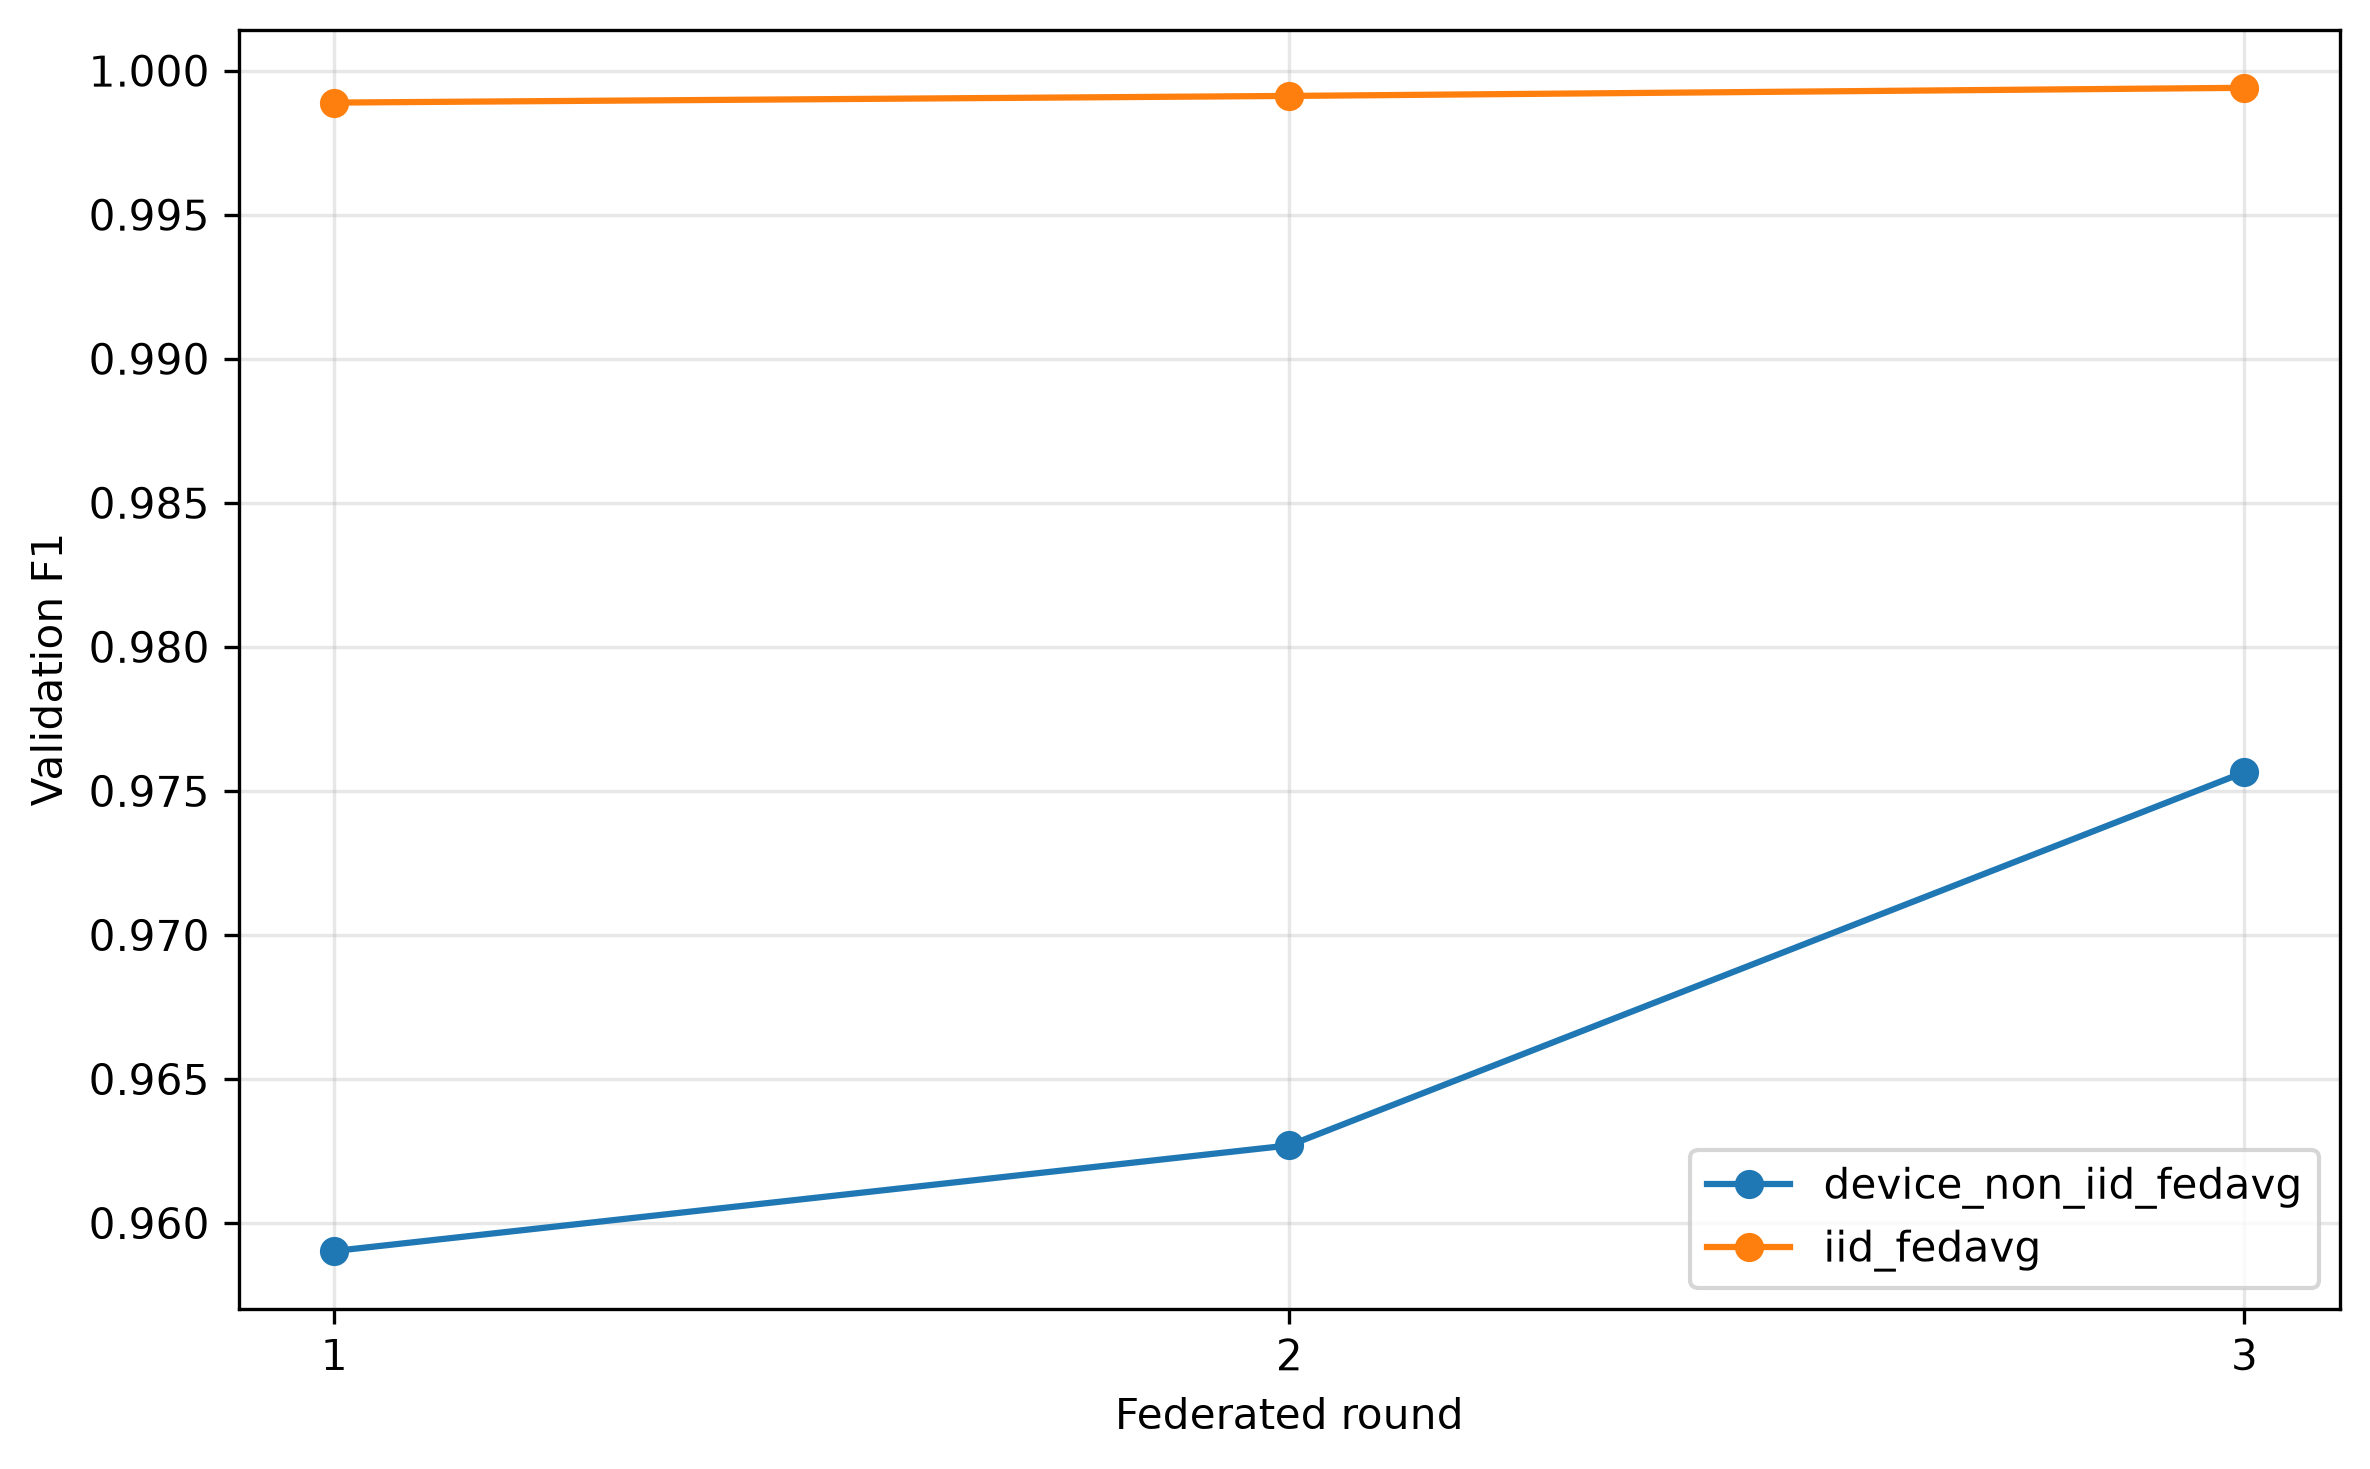
\includegraphics[width=\linewidth]{figures/fedavg_f1_convergence.png}
\caption{Validation F1-Score progression across communication rounds for Device Non-IID and Controlled IID FedAvg.}
\label{fig:f1_convergence}
\end{figure}

\begin{figure}[htbp]
\centering
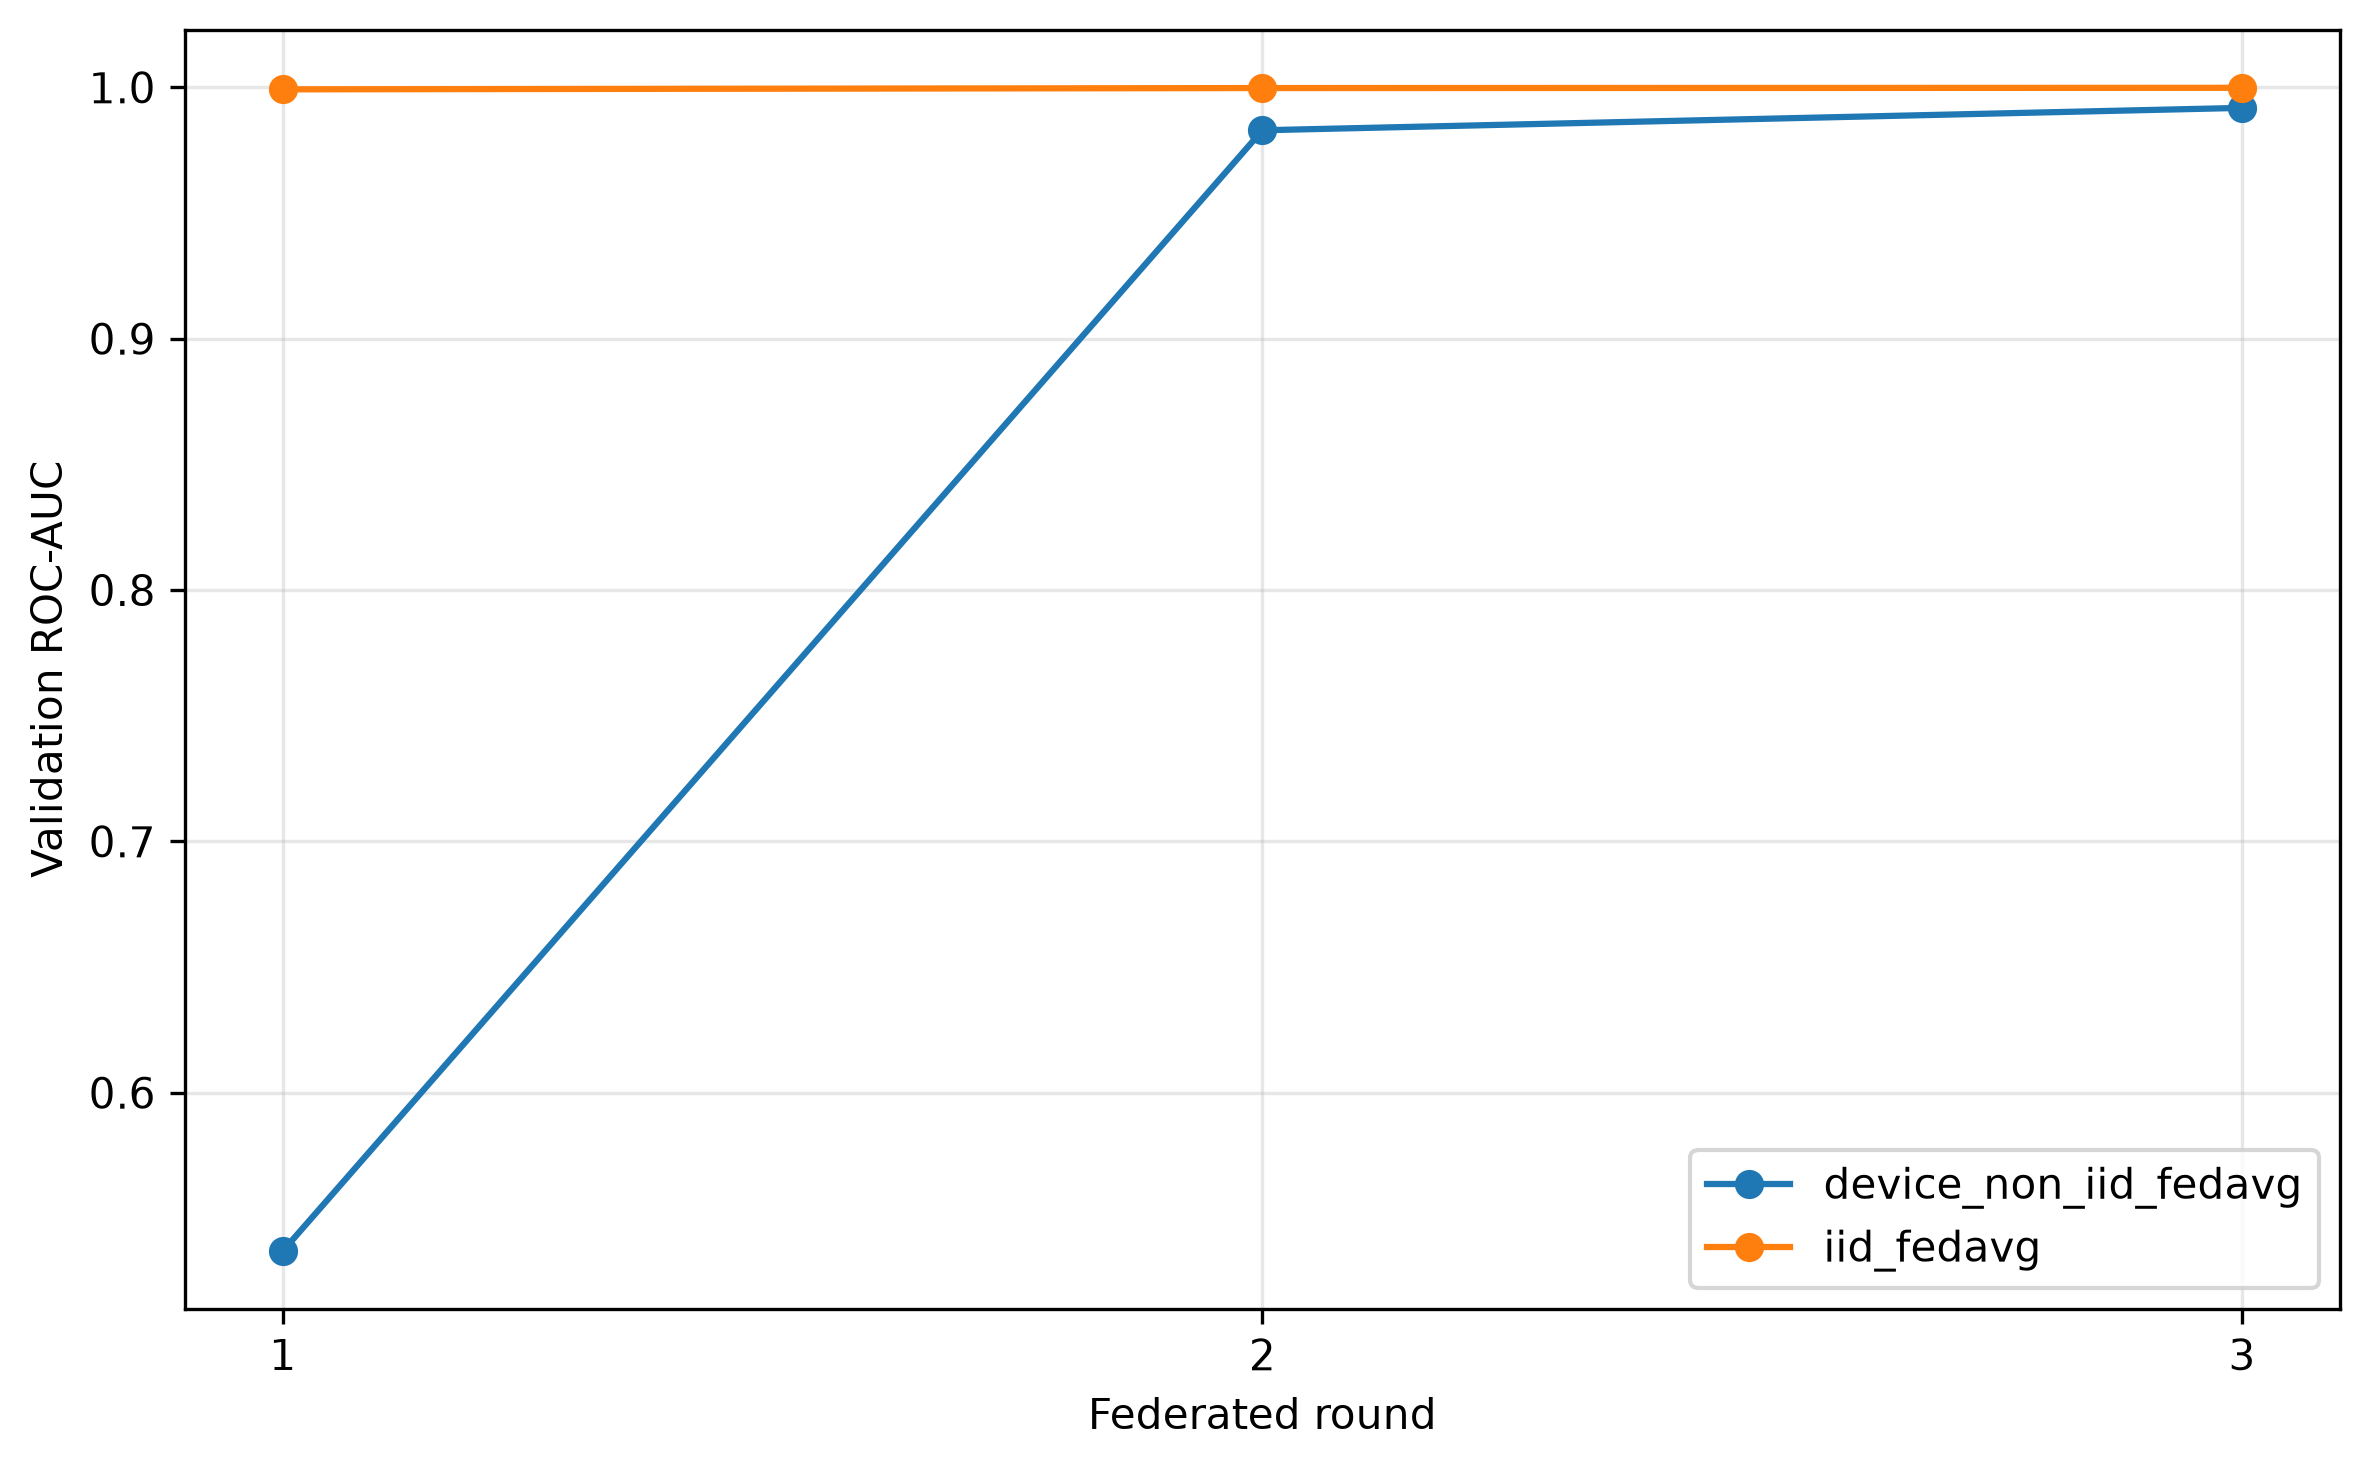
\includegraphics[width=\linewidth]{figures/fedavg_roc_auc_convergence.png}
\caption{Validation ROC-AUC progression across communication rounds for Device Non-IID and Controlled IID FedAvg.}
\label{fig:auc_convergence}
\end{figure}

\subsection{Local-Only Device-Level Results}
Table~\ref{tab:local_only} details per-device performance for Local-Only models.

\begin{table*}[t]
\caption{Local-Only model test evaluation performance by individual IoT device source.}
\label{tab:local_only}
\centering
\begin{tabular}{l c c c c c c c}
\toprule
\textbf{Device Identifier} & \textbf{Test Samples} & \textbf{Loss} & \textbf{Accuracy} & \textbf{Precision} & \textbf{Recall} & \textbf{F1-Score} & \textbf{ROC-AUC} \\
\midrule
\textbf{Danmini\_Doorbell} & 152,744 & 0.407299 & 0.951343 & 0.951343 & 1.000000 & 0.975065 & 0.987414 \\
\textbf{Ecobee\_Thermostat} & 125,381 & 0.061210 & 0.984320 & 0.984320 & 1.000000 & 0.992098 & 0.995744 \\
\textbf{Ennio\_Doorbell} & 53,325 & 0.758990 & 0.892339 & 0.892088 & 1.000000 & 0.942967 & 0.986173 \\
\textbf{Philips\_B120N10\_Baby\_Monitor} & 164,801 & 0.622557 & 0.840565 & 0.840555 & 1.000000 & 0.913371 & 0.997396 \\
\textbf{Provision\_PT\_737E\_Camera} & 124,239 & 0.356412 & 0.943971 & 0.942885 & 1.000000 & 0.970603 & 0.993009 \\
\textbf{Provision\_PT\_838\_Camera} & 125,533 & 0.535976 & 0.921264 & 0.918077 & 0.999991 & 0.957285 & 0.997157 \\
\textbf{Samsung\_SNH\_1011\_N\_Webcam} & 56,283 & 0.011711 & 0.997015 & 0.996647 & 0.999897 & 0.998269 & 0.999943 \\
\textbf{SimpleHome\_1002\_Camera} & 129,458 & 0.046649 & 0.987703 & 0.987254 & 0.999910 & 0.993542 & 0.999340 \\
\textbf{SimpleHome\_1003\_Camera} & 127,624 & 0.020290 & 0.999216 & 0.999255 & 0.999944 & 0.999599 & 0.993573 \\
\bottomrule
\end{tabular}
\end{table*}

\begin{figure}[htbp]
\centering
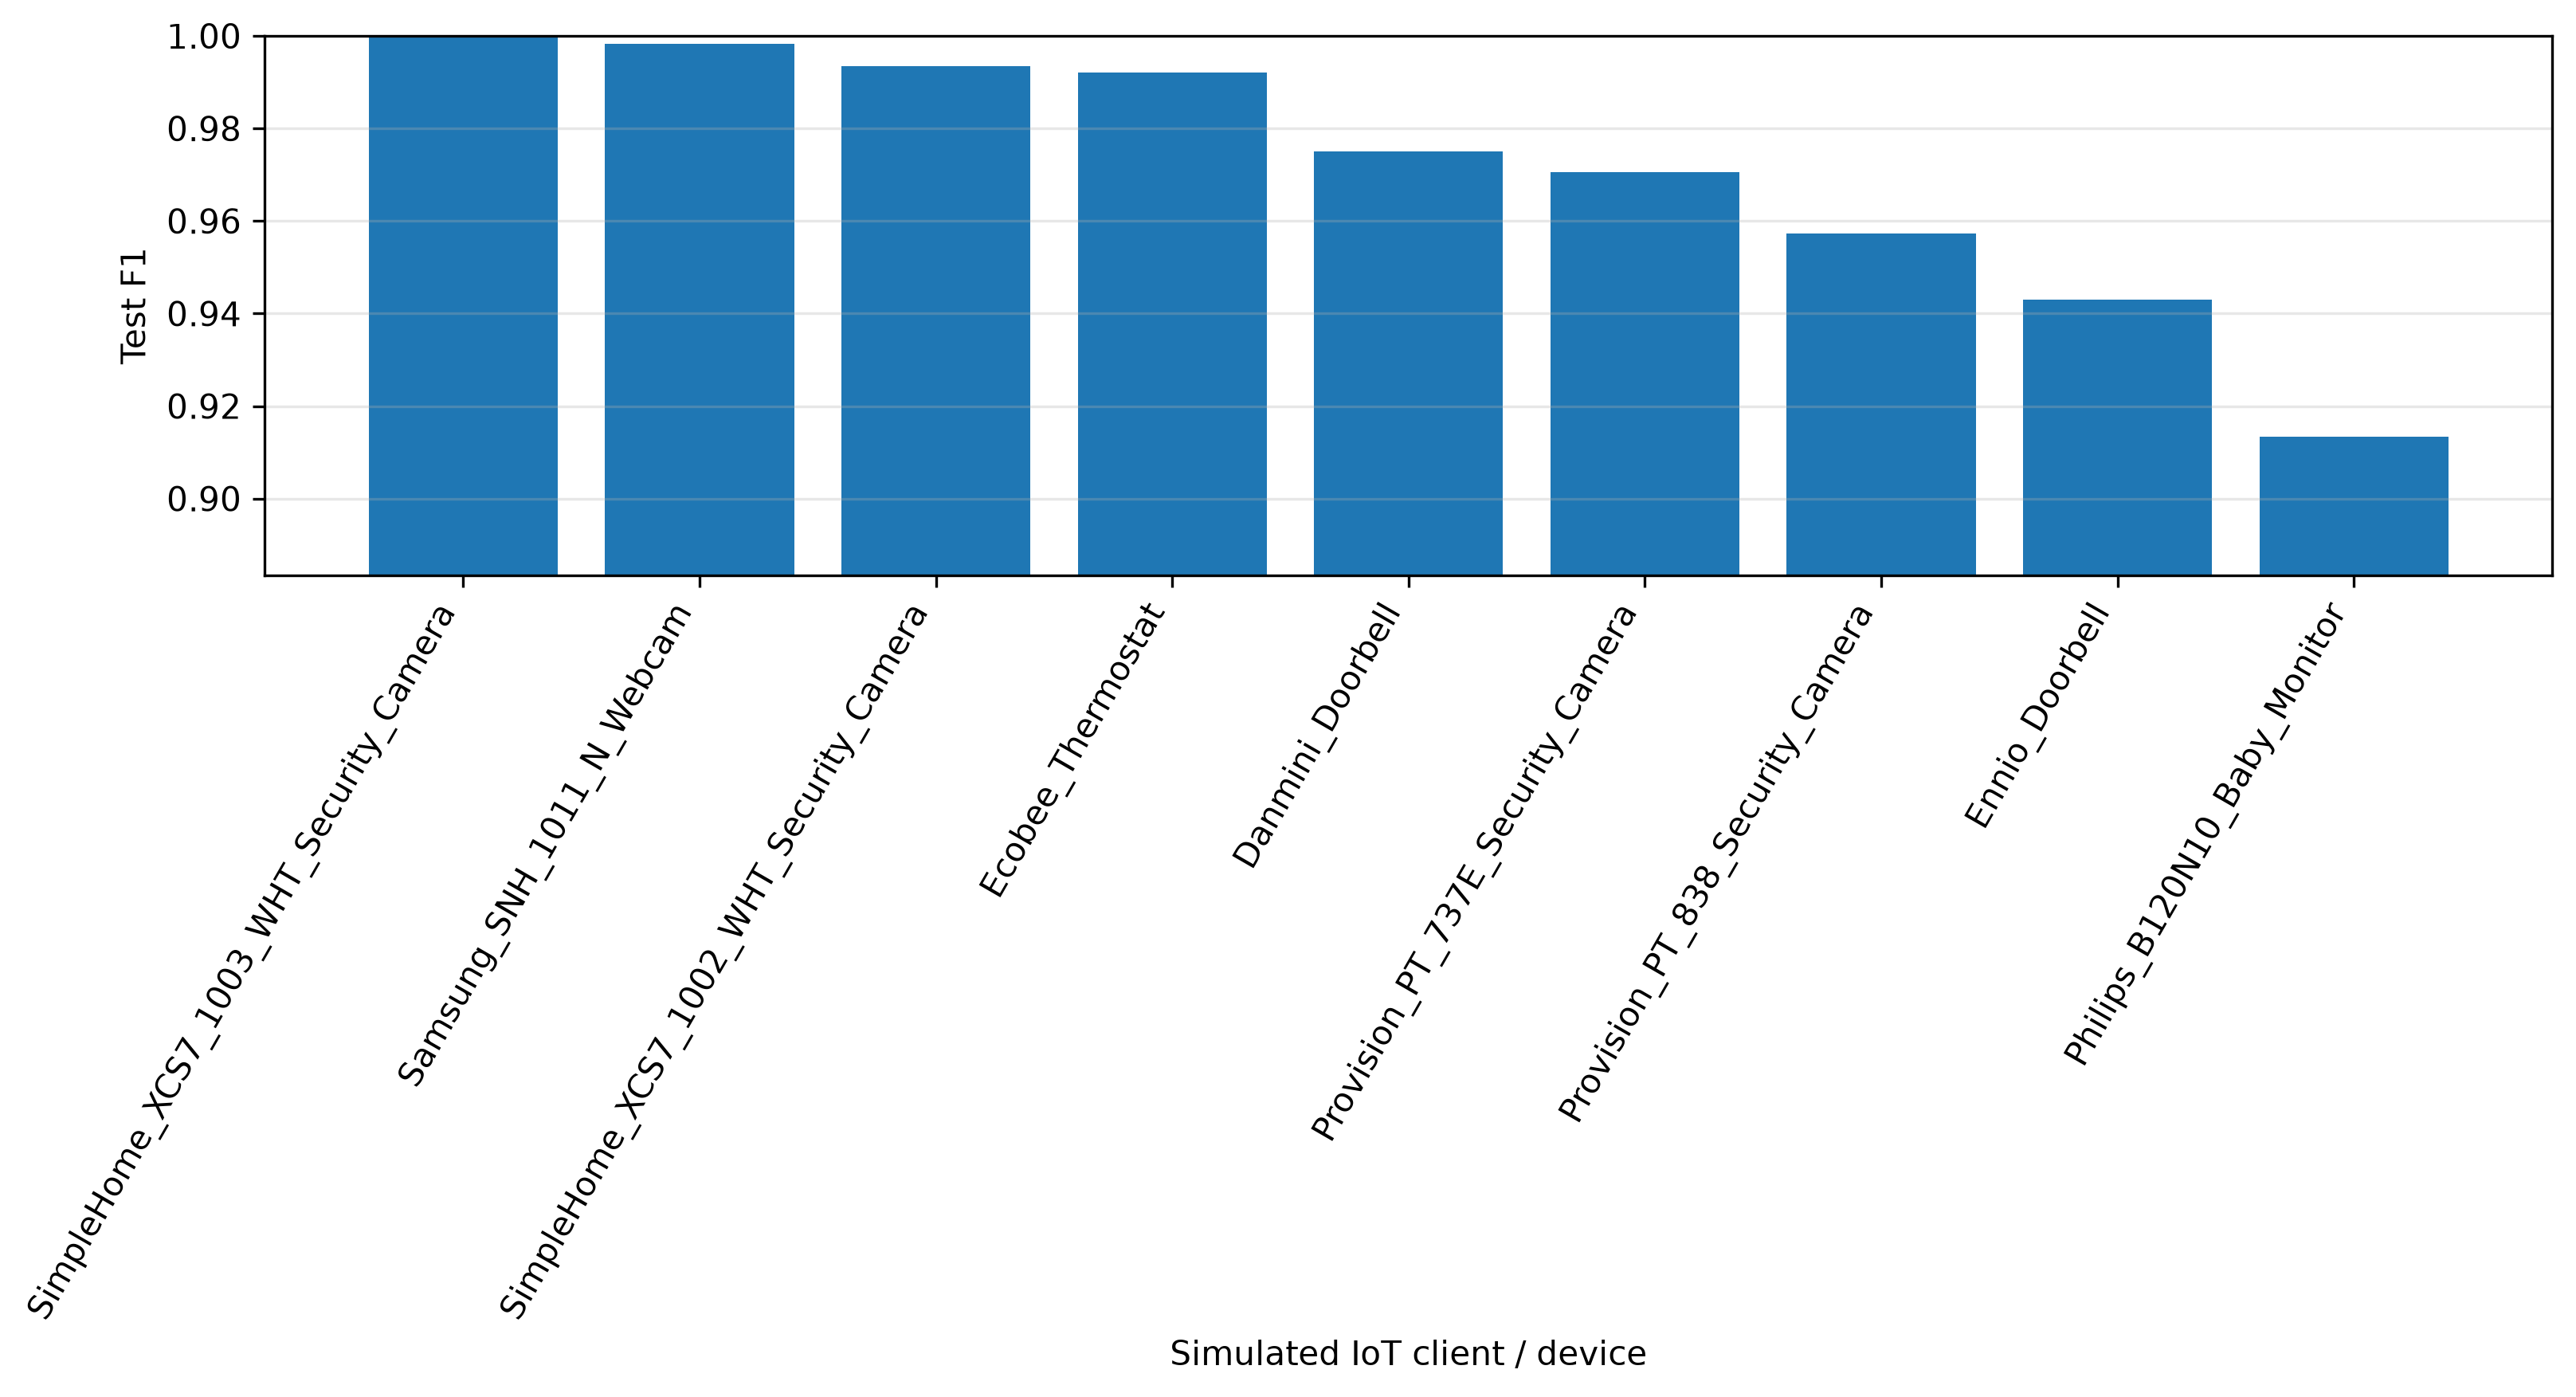
\includegraphics[width=\linewidth]{figures/local_only_f1_by_device.png}
\caption{Final test F1-Score breakdown for Local-Only models evaluated on individual device test partitions.}
\label{fig:local_only}
\end{figure}

\subsection{Communication Cost}
Table~\ref{tab:communication} details communication volume accounting.

\begin{table*}[t]
\caption{Model parameter payload communication volume accounting.}
\label{tab:communication}
\centering
\begin{tabular}{l c c c c c c}
\toprule
\textbf{Scenario} & \textbf{Rounds} & \textbf{Clients} & \textbf{Download (Bytes)} & \textbf{Upload (Bytes)} & \textbf{Total Exchange (Bytes)} & \textbf{Total (MiB)} \\
\midrule
\textbf{Per Client per Round} & 1 & 1 & 38,148 & 38,148 & 76,296 & 0.072762 \\
\textbf{All Clients per Round} & 1 & 9 & 343,332 & 343,332 & 686,664 & 0.654854 \\
\textbf{Measured 3-Round Experiment} & 3 & 9 & 1,029,996 & 1,029,996 & 2,059,992 & 1.964561 \\
\textbf{Configured 10-Round Projection} & 10 & 9 & 3,433,320 & 3,433,320 & 6,866,640 & 6.548538 \\
\bottomrule
\end{tabular}
\end{table*}

\begin{figure}[htbp]
\centering
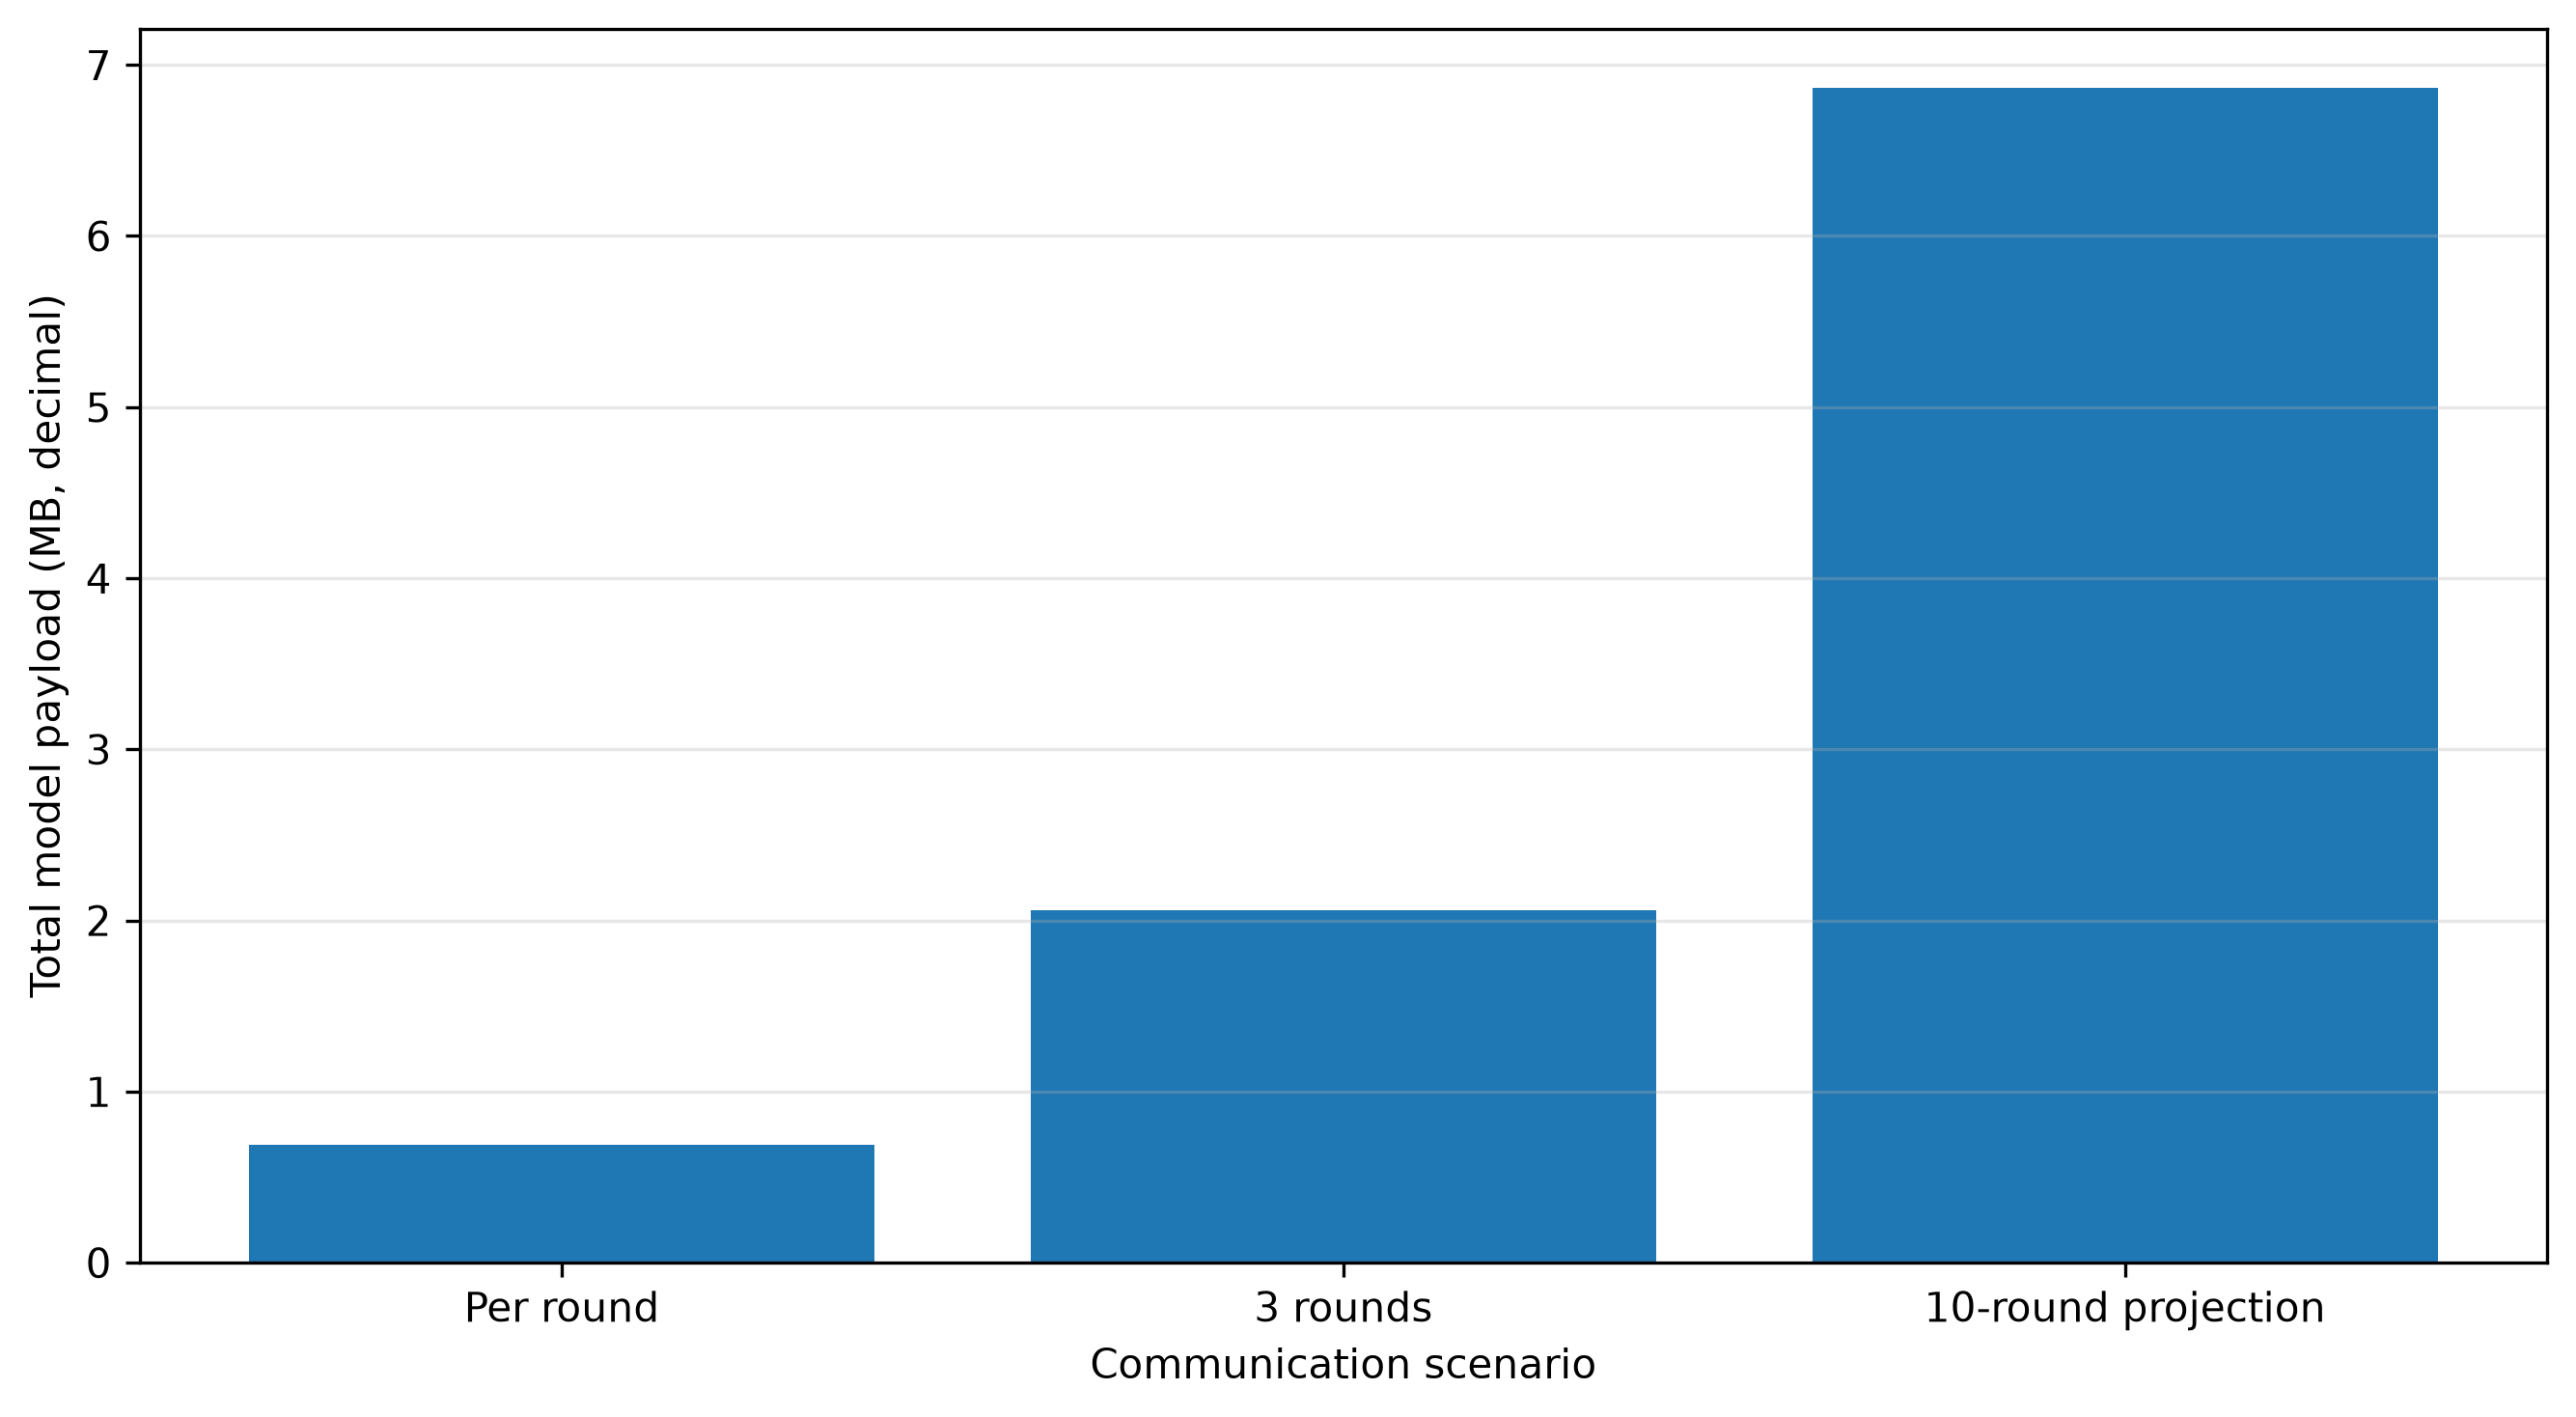
\includegraphics[width=\linewidth]{figures/communication_payload.png}
\caption{Cumulative model parameter payload transmission volume across communication rounds.}
\label{fig:communication}
\end{figure}

\subsection{Computational Resource Usage}
Table~\ref{tab:resources} presents execution runtimes and memory usage.

\begin{table*}[t]
\caption{Computational resource usage and wall-clock execution runtimes on CPU.}
\label{tab:resources}
\centering
\begin{tabular}{l c c c c c}
\toprule
\textbf{Experiment} & \textbf{Status} & \textbf{Peak RSS (Bytes)} & \textbf{Peak RSS (MiB)} & \textbf{Execution Wall Time (s)} & \textbf{Wall Time (Min)} \\
\midrule
\textbf{Centralized Baseline} & Completed & 640,614,400 & 610.9375 & 5,018.94 & ~83.65 min \\
\textbf{Local-Only Baseline} & Completed & 640,630,784 & 610.9531 & 3,402.99 & ~56.72 min \\
\textbf{Device Non-IID FedAvg} & Completed & 651,730,944 & 621.5391 & 4,034.84 & ~67.25 min \\
\textbf{Controlled IID FedAvg} & Completed & 700,821,504 & 668.3555 & 16,290.68 & ~271.51 min \\
\bottomrule
\end{tabular}
\end{table*}

\begin{figure}[htbp]
\centering
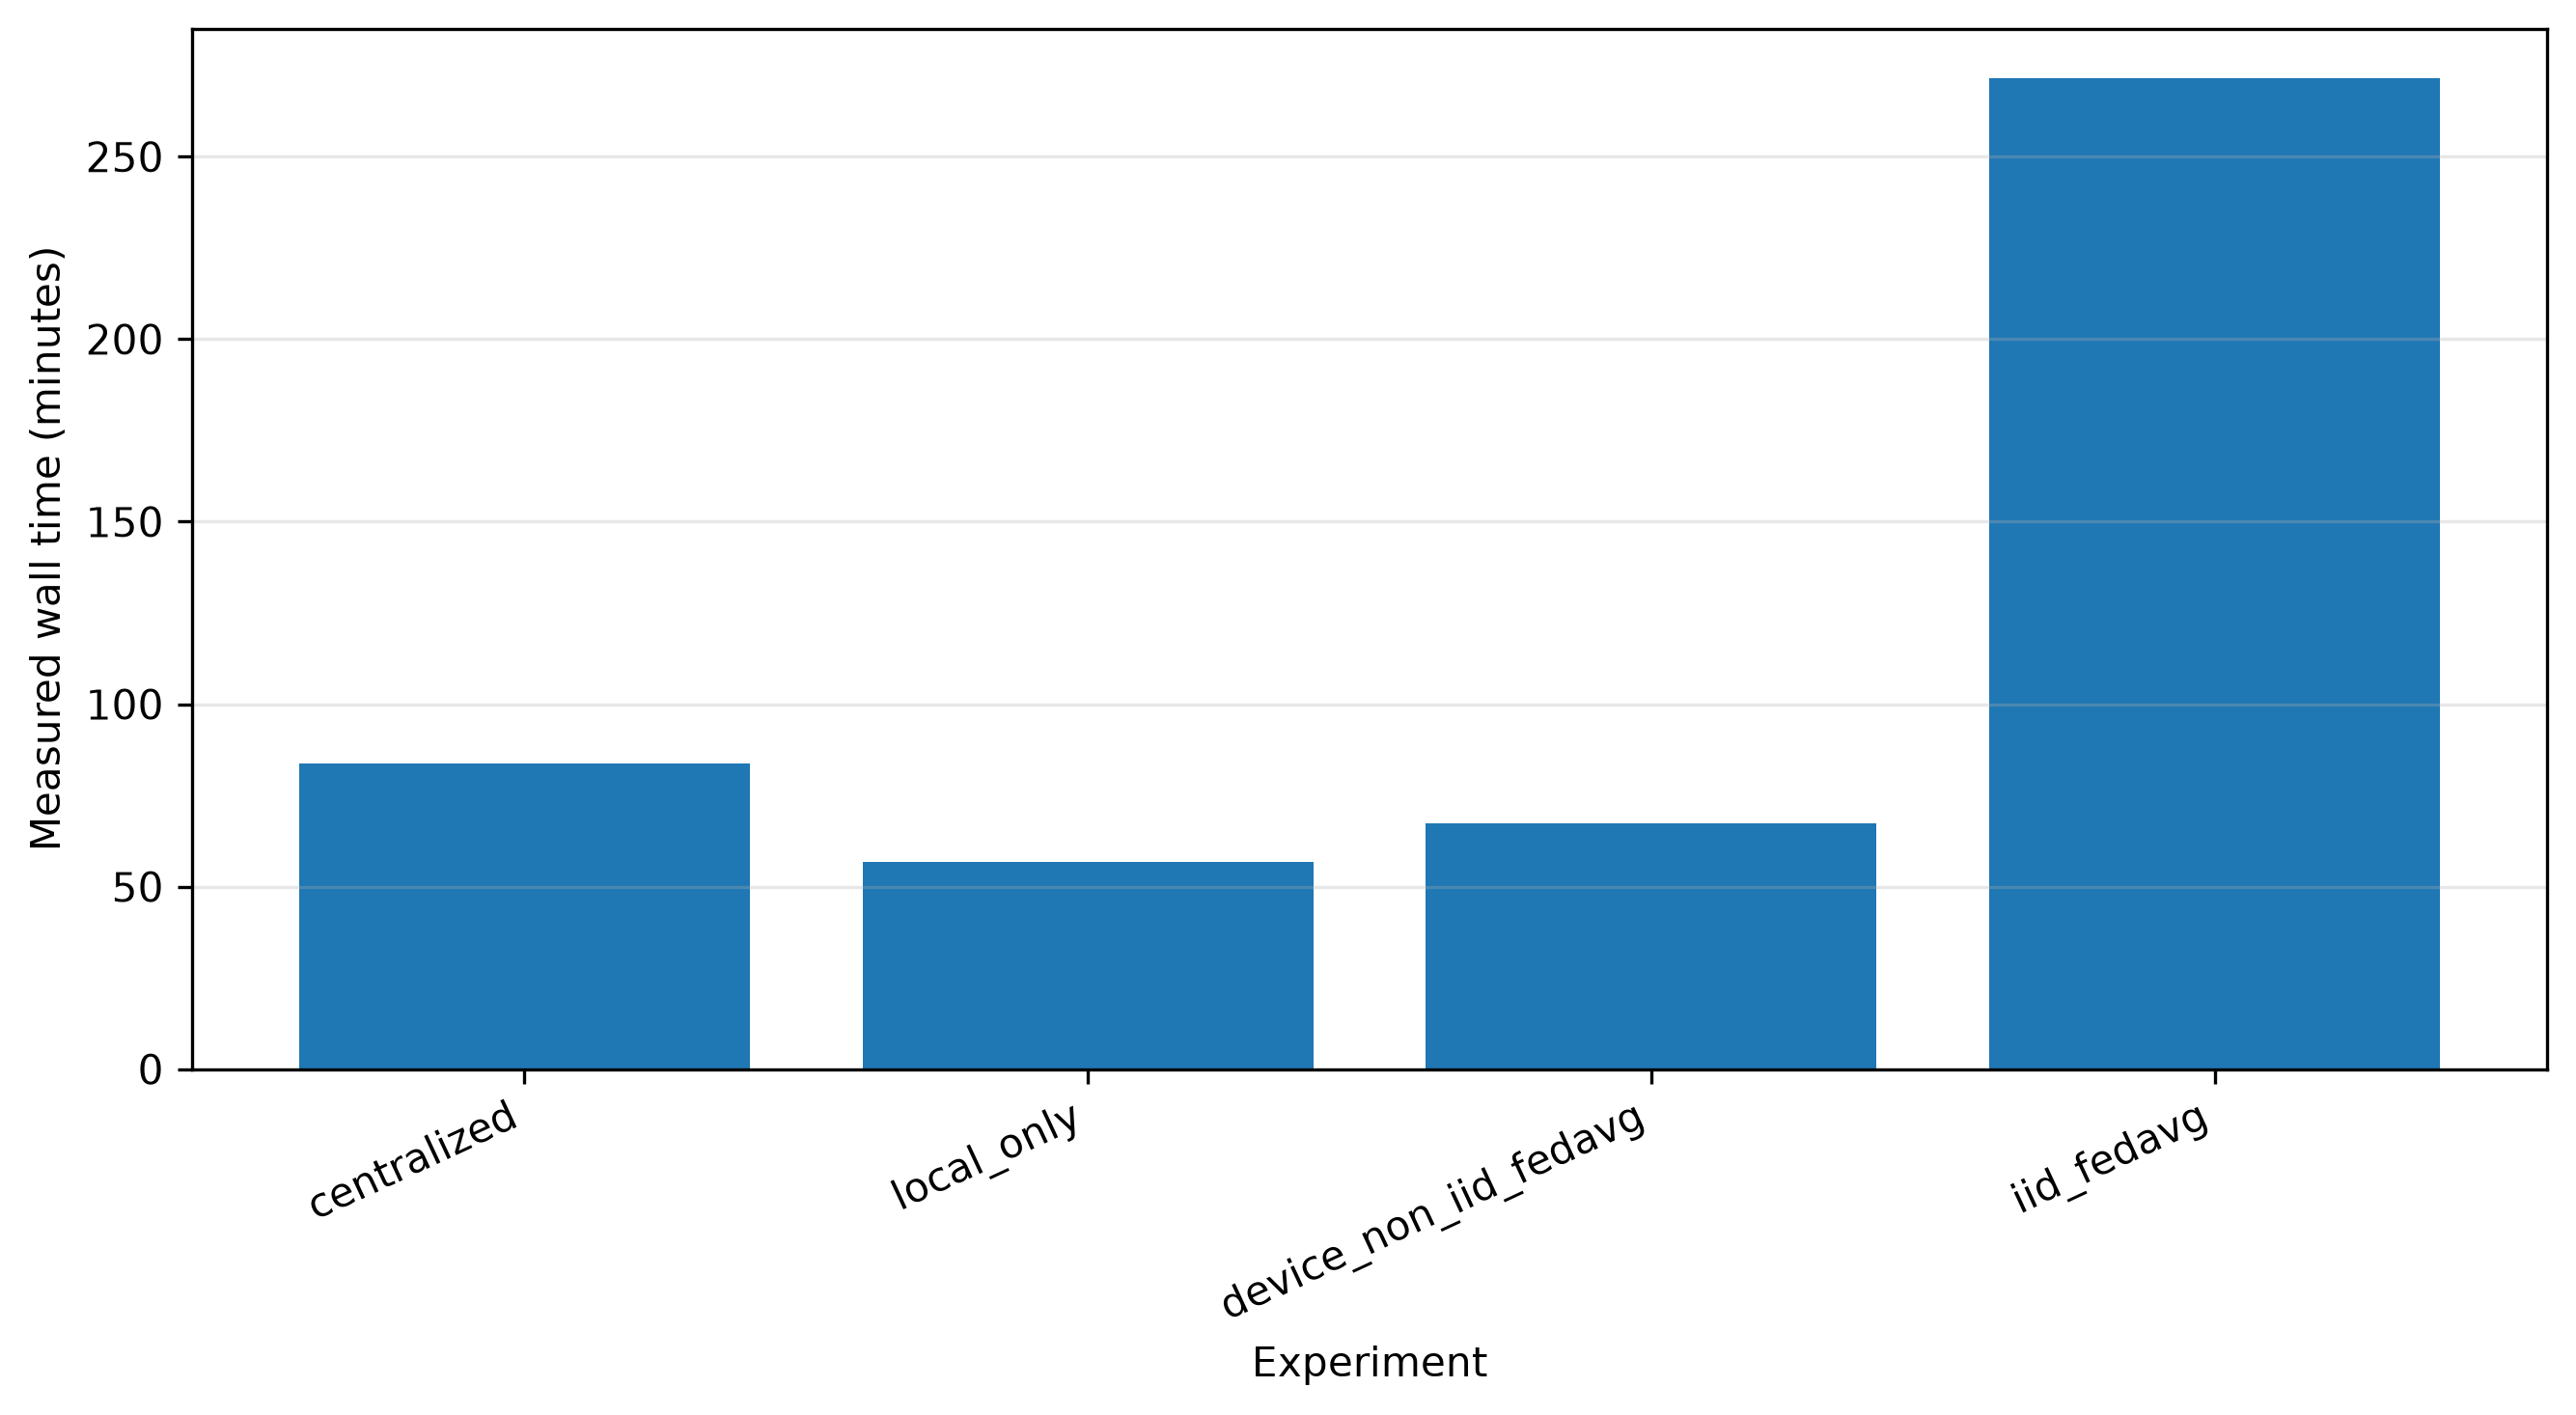
\includegraphics[width=\linewidth]{figures/experiment_runtime.png}
\caption{Total execution wall time across experimental conditions on CPU.}
\label{fig:runtime}
\end{figure}

\begin{figure}[htbp]
\centering
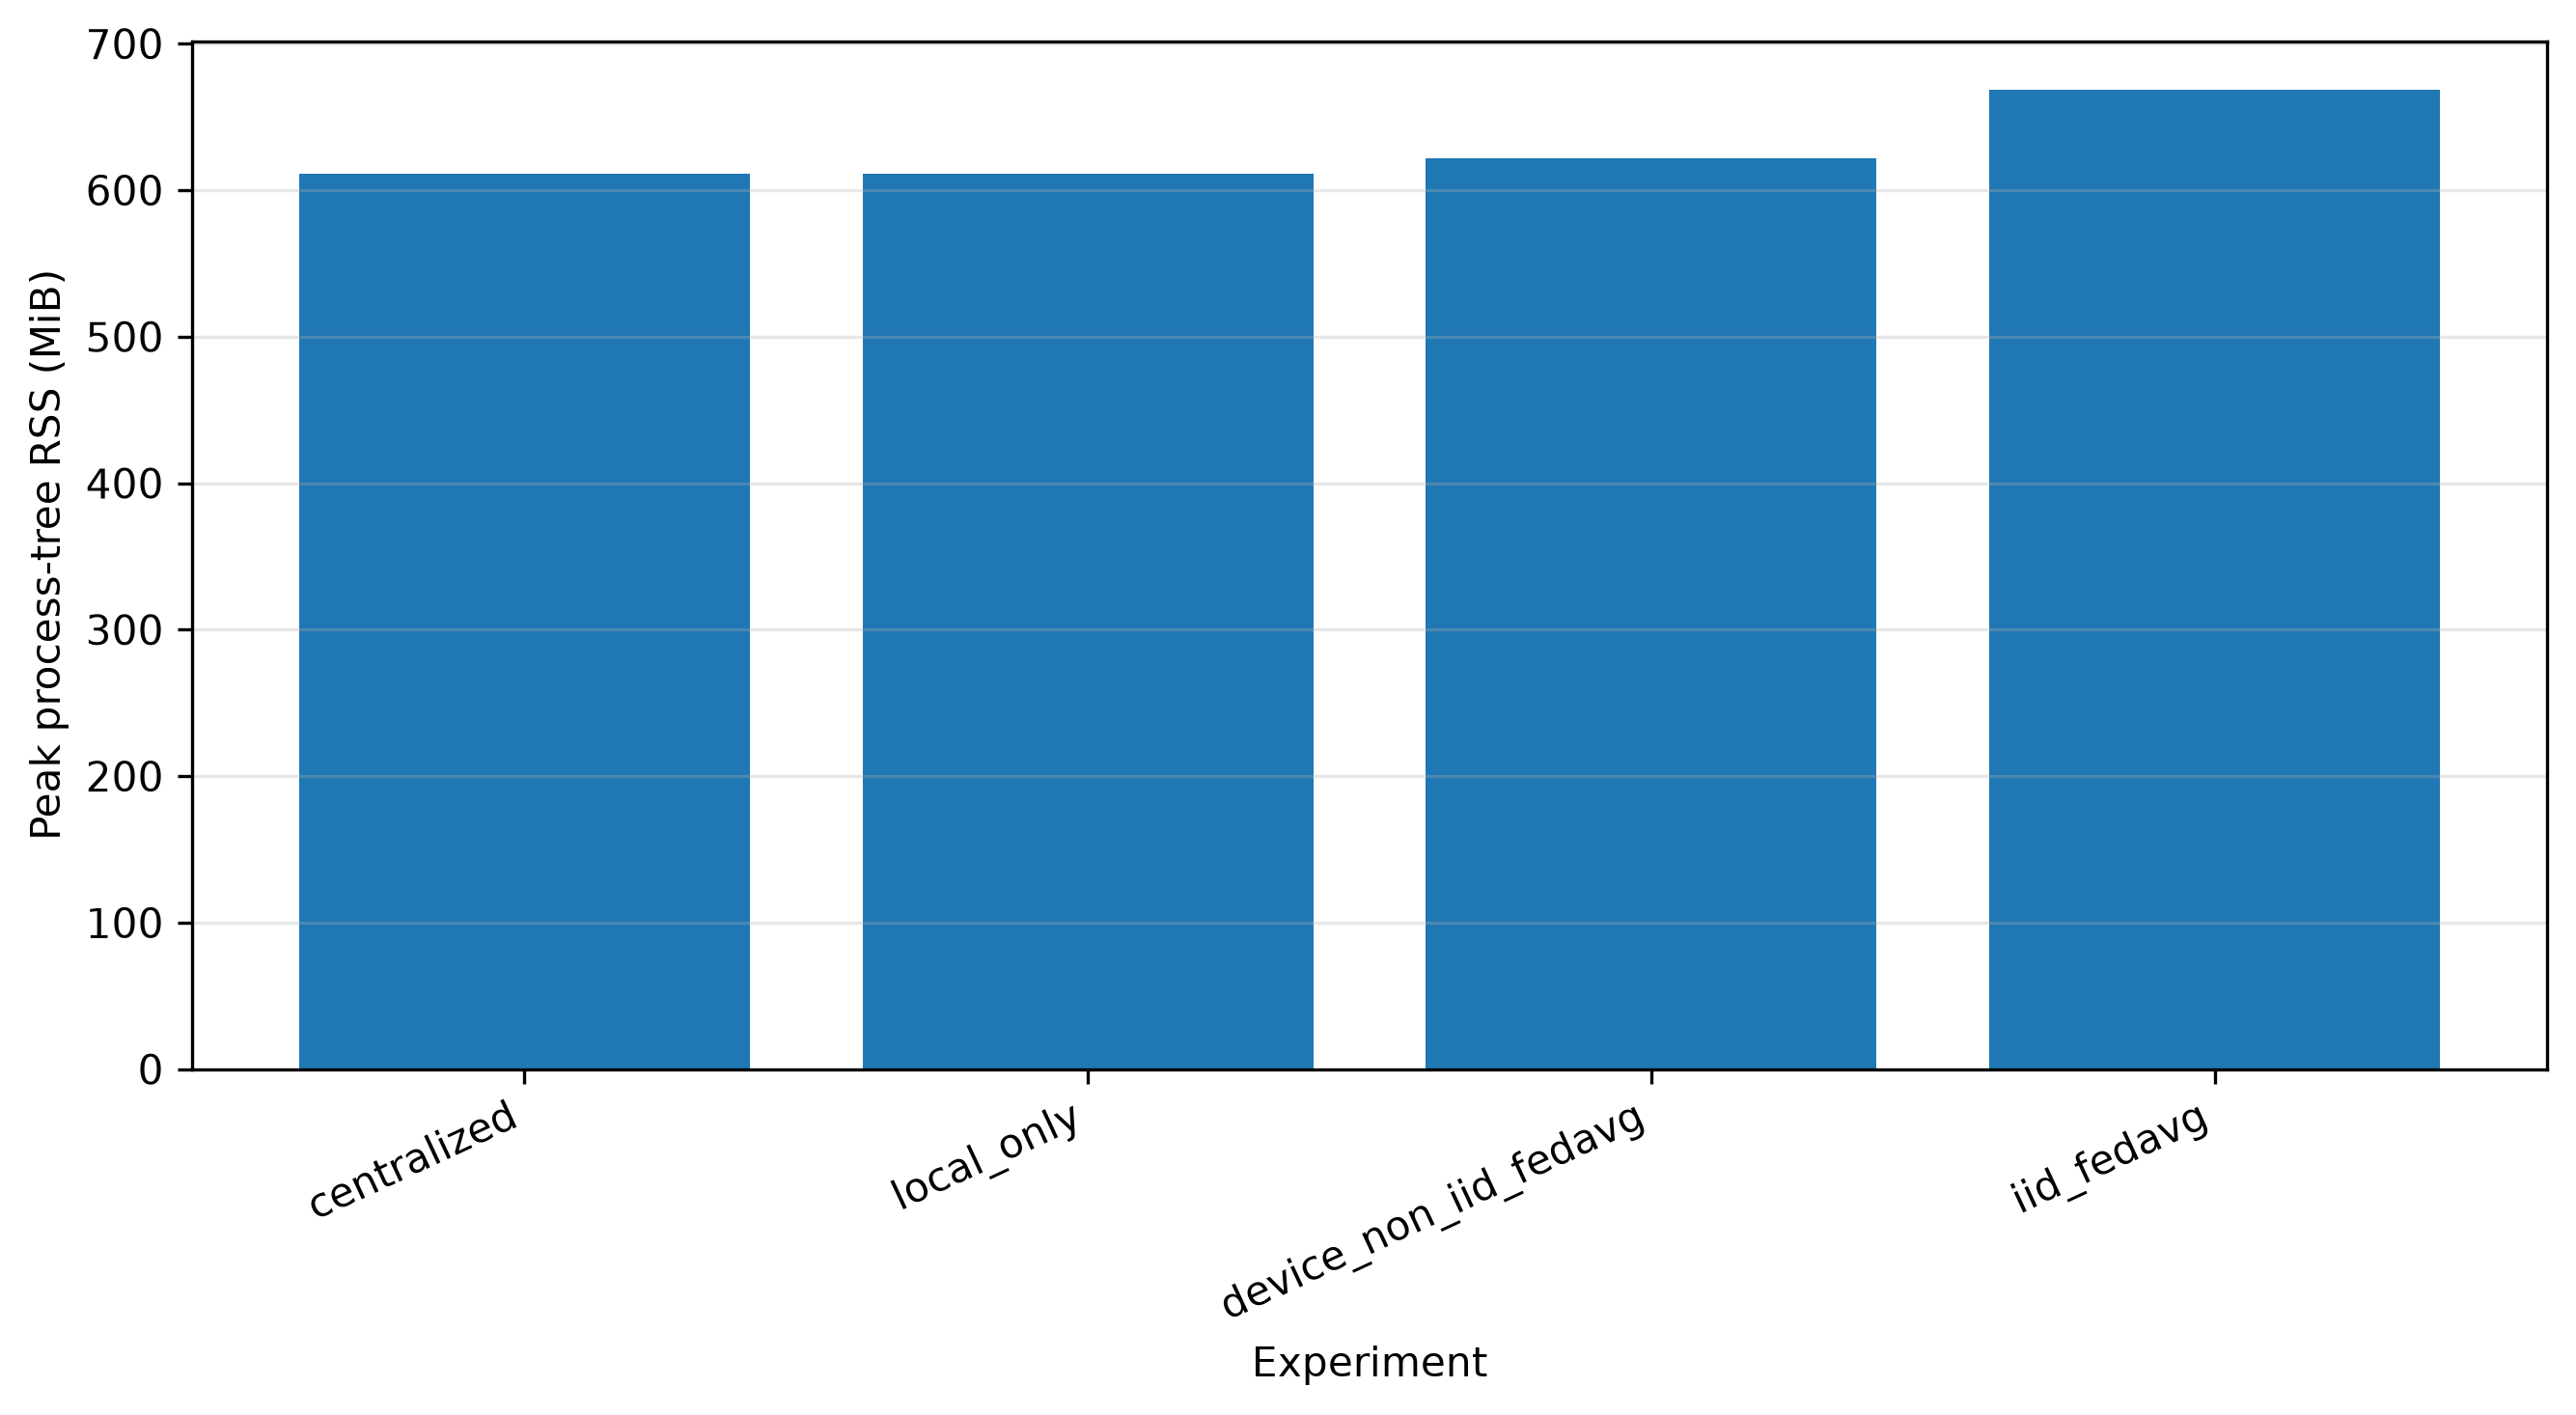
\includegraphics[width=\linewidth]{figures/peak_memory_usage.png}
\caption{Observed peak process-tree RAM usage (Resident Set Size in MiB) across experimental conditions.}
\label{fig:memory}
\end{figure}

\section{Discussion}
\label{sec:discussion}
The empirical results demonstrate clear trade-offs across training topologies. Controlled IID partitioning yielded global test metrics matching the centralized benchmark (F1: 0.9994 vs. 0.9971), whereas natural device-level Non-IID partitioning reached F1 = 0.9757. Local-Only models exhibited significant precision variations across devices (0.8406 to 0.9993). Compact parameter payload size (38,148 bytes/transfer) minimizes communication requirements but does not eliminate local computational execution runtime on host CPUs.

\section{Limitations and Threats to Validity}
\label{sec:limitations}
Key limitations include: single random seed execution (seed 42), 3-round execution window, simulated single-host CPU execution, centrally pre-fitted feature standardization scaler, theoretical model weight payload accounting rather than socket-level traffic measurement, and absence of formal privacy-preserving primitives (Differential Privacy / Secure Aggregation) or adversarial robustness evaluations.

\section{Conclusion and Future Work}
\label{sec:conclusion}
\label{sec:future_work}
This study presented a controlled empirical investigation of federated learning for IoT intrusion detection using the N-BaIoT dataset. The compact \texttt{SmallMLP} architecture achieved high detection performance while requiring ~1.96 MiB of cumulative parameter exchange over 3 rounds across 9 clients. Future work includes multi-seed statistical evaluation, extended round convergence analysis, federated preprocessing protocols, alternative non-IID algorithms (FedProx/SCAFFOLD), and physical edge hardware deployments.

\bibliographystyle{IEEEtran}
\bibliography{references}

\end{document}
